%%%%%%%%%%%%%%%%%%%%%%%%%%%%%%%%%%%%%%%%%
% Medium Length Graduate Curriculum Vitae
% LaTeX Template
% Version 1.1 (9/12/12)
%
% This template has been downloaded from:
% http://www.LaTeXTemplates.com
%
% Original author:
% Rensselaer Polytechnic Institute (http://www.rpi.edu/dept/arc/training/latex/resumes/)
%
% Modified By:
% Oscar Neiva
% oscar-neiva.github.io 
% oscarneivaeneto@gmail.com
%
% Important note:
% This template requires the res.cls file to be in the same directory as the
% .tex file. The res.cls file provides the resume style used for structuring the
% document.
%
%%%%%%%%%%%%%%%%%%%%%%%%%%%%%%%%%%%%%%%%%

%----------------------------------------------------------------------------------------
%	PACKAGES AND OTHER DOCUMENT CONFIGURATIONS
%----------------------------------------------------------------------------------------

\documentclass[margin, 10pt]{res} % Use the res.cls style, the font size can be changed to 11pt or 12pt here
\usepackage{graphics}
\usepackage{epsfig}
\usepackage{helvet} % Default font is the helvetica postscript font
\usepackage[utf8]{inputenc}
%\usepackage{newcent} % To change the default font to the new century schoolbook postscript font uncomment this line and comment the one above
%\usepackage[lmargin=2.5cm,rmargin=2cm,tmargin=2cm,bmargin=2cm]{geometry}
\setlength{\textwidth}{5.1in} % Text width of the document

\begin{document}

%----------------------------------------------------------------------------------------
%	NAME AND ADDRESS SECTION
%----------------------------------------------------------------------------------------
\moveleft\hoffset\vbox{\hrule width\resumewidth height 1pt}\smallskip %

\vspace{-0.2cm}
\hspace{-3.0cm}
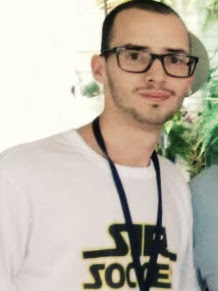
\includegraphics[width=2.2cm]{figures/profile.jpg}

\vspace{-3cm}
\leftline{\large\bf Oscar Neiva} % Your name at the top
\vspace{0.5cm}
\leftline{oscarneivaeneto@gmail.com}
\leftline{oscar-neiva.github.io}
\leftline{Rio de Janeiro, RJ}
 
\vspace{0.8cm}

\moveleft\hoffset\vbox{\hrule width\resumewidth height 1pt}\smallskip % Horizontal line after name; adjust line thickness by changing the '1pt'
 


%----------------------------------------------------------------------------------------

\begin{resume}

%----------------------------------------------------------------------------------------
%	Objective and Interest
%----------------------------------------------------------------------------------------
 
%\section{Objective and Interest}  

%A intership in the field of software development. 

%----------------------------------------------------------------------------------------
%	Experience
%----------------------------------------------------------------------------------------
 
\section{Experience}

{\sl Scientific Internship} \hfill May of 2014 - March of 2016\\
Laboratório Nacional de Computação Científica - LNCC, Petrópolis, RJ 
\begin{itemize} \itemsep -2pt % Reduce space between items
\item At the LNCC my work was motivated by the study and simulation of systems subject to Markov jumps. The end goal was apply the concepts of Markov jump linear systems in a simulation of the PageRank algorithm, the algorithm behind the Google search engine.
\end{itemize}

{\sl Internship in Software Development} \hfill April of 2014 - December of 2015\\
Laboratório de Sistemas Inteligentes e Robótica - SIRLab, Petrópolis, RJ 
\begin{itemize} \itemsep -2pt % Reduce space between items
\item At the SIRLab I worked as software developer in C++ language. The project which I was part of had consisted in develop a autonomous system to guide and control mobile robots. Among the parts of the SIRSoccer system development I was in charge of find and study a control model adequate for the system and create an algorithm with such model.
\end{itemize}

%----------------------------------------------------------------------------------------
%	Education
%----------------------------------------------------------------------------------------

\section{Education}

Faculdade de Educação Tecnológica do Estado do Rio de Janeiro - FAETERJ \\
{\sl Technologist,} Information Technology, Petrópolis, RJ, 2013 - 2016.

Colégio M3 \\
College, Niterói, RJ, 2009 - 2011.
 
%----------------------------------------------------------------------------------------
%	Languages
%----------------------------------------------------------------------------------------

\section{Languages}
{\sl Portuguese,} Native.\\
{\sl English,} Advanced.

%----------------------------------------------------------------------------------------
%	Skills
%----------------------------------------------------------------------------------------

\section{Skills} 

{\sl Languages \& Software:} C, C++, Linux, OpenGL, OpenCV, Arduino, Matlab, Octave, LaTeX, Java, PHP, HTML, CSS, Microsoft Excel.

{\sl Others:} Systems and Control Theory, Real-time Control Systems, Search Engine Optimisation - SEO, Stochastic Processes.
 
%----------------------------------------------------------------------------------------
%	Courses and Extra-Curricular Activities
%----------------------------------------------------------------------------------------

\section{Courses and Extra-Curricular Activities} 
X Escola Luso-Brasileira de Computação Evolutiva, LNCC, February 2014\\
IX Escola de Verão do Laboratório Associado de Computação e Matemática Aplicada, INPE, February 2015\\
Processos de Lévy Aplicados a Finança, LNCC, January 2015\\

%----------------------------------------------------------------------------------------
%	Awards
%----------------------------------------------------------------------------------------

\section{Awards} 
RUNNER-UP in category RoboCup Simulation 2D, LARC/CBR, October 23, 2014.\\
Destaque na Jornada de Iniciação Científica e Tecnológica, LNCC, Setembro, 2015.

%----------------------------------------------------------------------------------------
%	Volunteer Work
%---------------------------------------------------------------------------------------- 

\section{Volunteer Work}

Referee at the Brazilian Robotics Olympiad (state Rio de Janeiro), august 2014\\
Organiser at the Brazilian Robotics Olympiad (local Petrópolis), august 2015

%----------------------------------------------------------------------------------------

\end{resume}
\end{document}